% arara: pdflatex
\documentclass{article}
%\usepackage[spanish,activeacute]{babel}
%\usepackage[english,activeacute]{babel}
%\usepackage[latin1]{inputenc}
\usepackage[utf8]{inputenc}
\usepackage[english]{babel}

\usepackage{amsmath,amsfonts,amssymb,amstext,amsthm,amscd}
\usepackage{hyperref}
\usepackage{latexsym}
\usepackage{graphicx}
%\usepackage{subfigure}
\usepackage{subfig}
%\linespread{1.6}
\usepackage{float}
\usepackage{dcolumn}% Align table columns on decimal point(esto lo saque del ejemplo de revtex4)
\usepackage{bm}% bold math(esto lo saque del ejemplo de revtex4)
\newcounter{itemR}
\usepackage{here} %recordar usar el comando[H] para las gráficas que es el comando here en lugar de [h!]
\usepackage{fancyhdr}
\usepackage{fancybox}
%\usepackage{sidecap}
%\usepackage[spanish,activeacute]{babel}
\usepackage{multirow}
\usepackage{multicol}
\usepackage{array}
\usepackage{enumitem}
\usepackage{listings}
\usepackage{xcolor}
%\usepackage{booktabs}% para hacer tablas profesionales con \toprule


\lstset{
  language={Java},
  basicstyle=\footnotesize,  % El tamaño de la fuente que se usa para el código
  keywordstyle=\color{blue}, 
  commentstyle=\color{gray},
  stringstyle=\color{orange},
  numbers=left,  % Dónde poner los números de línea
  numberstyle=\footnotesize,  % El tamaño de la fuente que se usa para los números de línea
  stepnumber=1,  % El paso entre dos números de línea
}

\makeatletter
\newenvironment{CenteredBox}{%
\begin{Sbox}}{%
\end{Sbox}\centerline{\parbox{\wd\@Sbox}{\TheSbox}}}% Y lo centra
\makeatother
% ----------

\usepackage{fancyhdr}
\setlength{\headheight}{15.2pt}
\usepackage[paperwidth=8.5in, paperheight=11.0in, top=1.0in, bottom=1.0in, left=1.0in, right=1.0in]{geometry}
\lstnewenvironment{code}{\lstset{basicstyle=\ttfamily}}{}

\pagestyle{fancyplain}
\fancyhead[LE,RO]{Reporte Dijkstra}
\fancyhead[CE,CO]{}
\fancyhead[RE,LO]{O23-LIS2012-1}
\fancyfoot[LE,RO]{\thepage}
\fancyfoot[CE,CO]{Matemáticas discretas, UDLAP}
\fancyfoot[RE,LO]{}

% -----------
\begin{document}
\fancypagestyle{plain}{
   	\renewcommand{\headrulewidth}{1pt}
   	\renewcommand{\footrulewidth}{1pt}
}
\renewcommand{\footrulewidth}{1pt}
\renewcommand{\tablename}{Tabla}
\renewcommand{\figurename}{Figura}


\title{Que necesita el sur-sureste para desarrollarse?}
\author{\small{Erick Gonzalez Parada ID: 178145}\\
	   \small{Matemáticas discretas, Universidad de las Américas Puebla, Puebla, M\'exico}}
\date{\small{\today}}
\maketitle

% ---------------
\begin{abstract}
Análisis de Dijkstra.\\
\\
\\
{\it Keywords:}   lista, adjacencia, vertices y aristas   
\\
\\
\end{abstract}

%-----------------
\section{Introducción}\label{Introducción}
El sur-sureste de México enfrenta desafíos significativos en términos de conexiones e infraestructura. La región se ve afectada por la falta de una red vial bien desarrollada, limitaciones en las conexiones ferroviarias, desigualdades en el desarrollo, carencias en la conectividad digital, necesidades en la infraestructura portuaria, desafíos topográficos, falta de inversiones y problemas socioeconómicos. Estos problemas, combinados, dificultan el desarrollo económico y social integral de la región. La superación de estos desafíos requerirá un enfoque integral que involucre inversiones significativas, planificación estratégica y coordinación entre diferentes niveles de gobierno y partes interesadas, mi objetivo es confirmar la desventaja de desconeccion que tiene esta región de Mexico

Además de los desafíos mencionados, es importante destacar que la región sur-sureste de México a menudo enfrenta dificultades relacionadas con la falta de acceso a servicios básicos, como educación y salud, lo que contribuye a la brecha socioeconómica. La planificación y ejecución de proyectos de infraestructura deben abordar estas necesidades fundamentales para lograr un desarrollo equitativo. Asimismo, la consideración de factores ambientales y sostenibles es esencial para mitigar impactos negativos en la ecología local.
\subsection*{Dijkstra en Java}
Nota: lo que se encuentra en el main de los fragmentos es una prueba de que el código funciona. 
\begin{figure}[H]
  \centering
  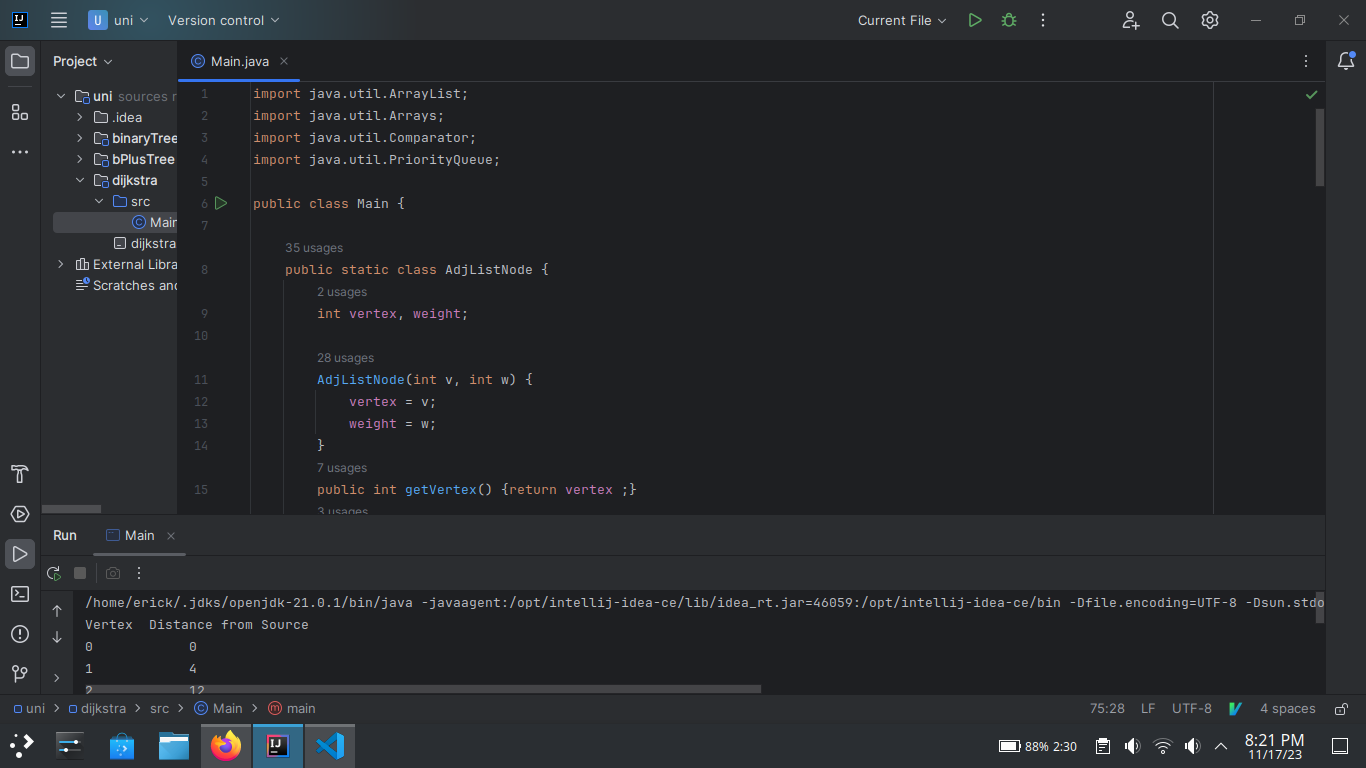
\includegraphics[scale=0.4]{../imgs/c.png}
  \caption{code fragment 1}
  \label{fig:1}
\end{figure}

\begin{figure}[H]
  \centering
  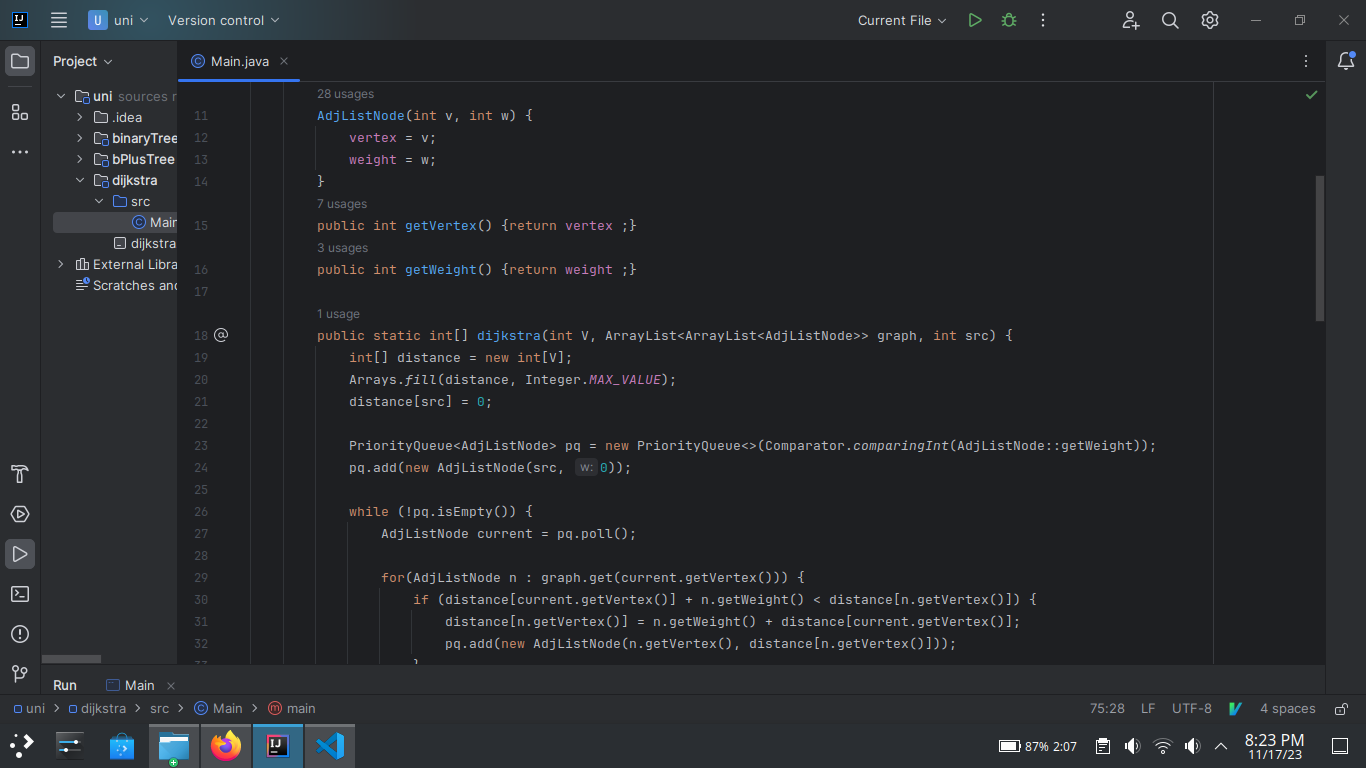
\includegraphics[scale=0.4]{../imgs/c1.png}
  \caption{code fragment 2}
  \label{fig:2}
\end{figure}

\begin{figure}[H]
  \centering
  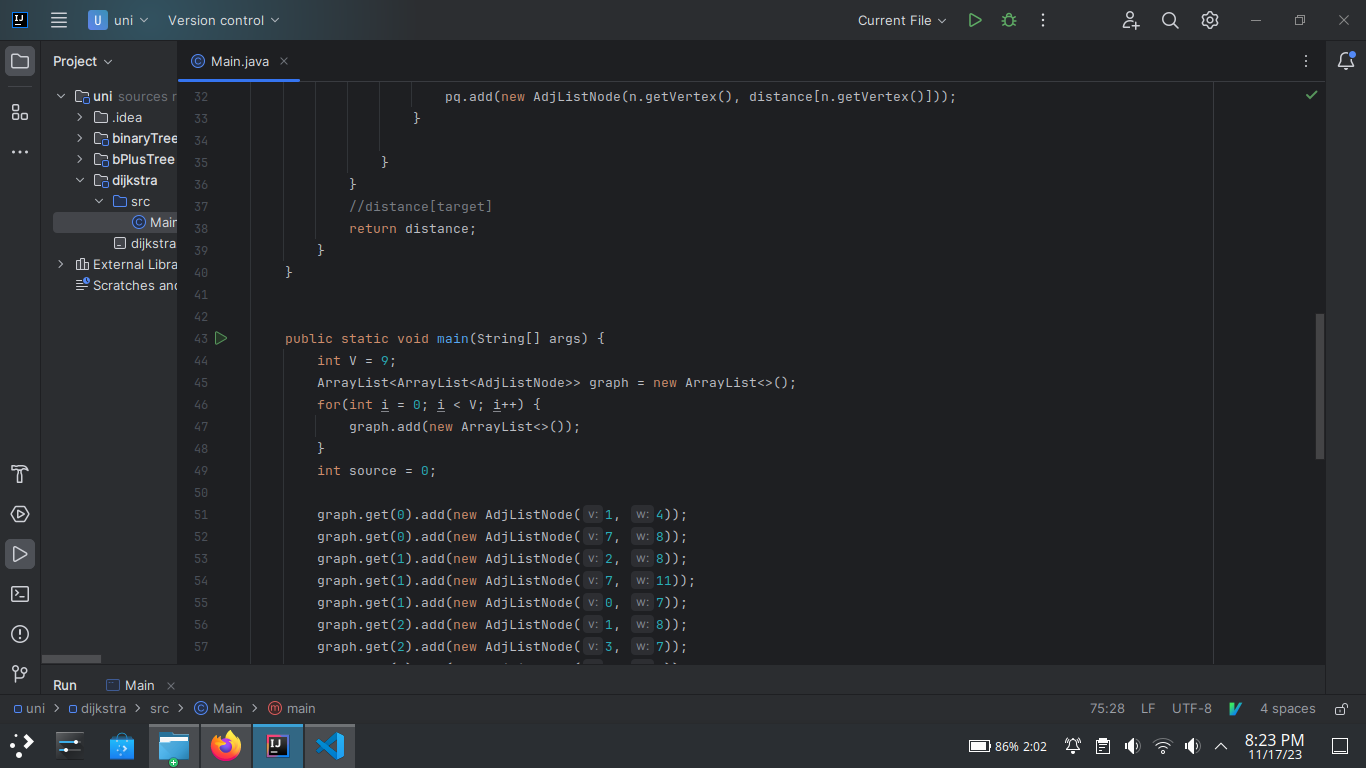
\includegraphics[scale=0.4]{../imgs/c2.png}
  \caption{code fragment 3}
  \label{fig:3}
\end{figure}

\begin{figure}[H]
  \centering
  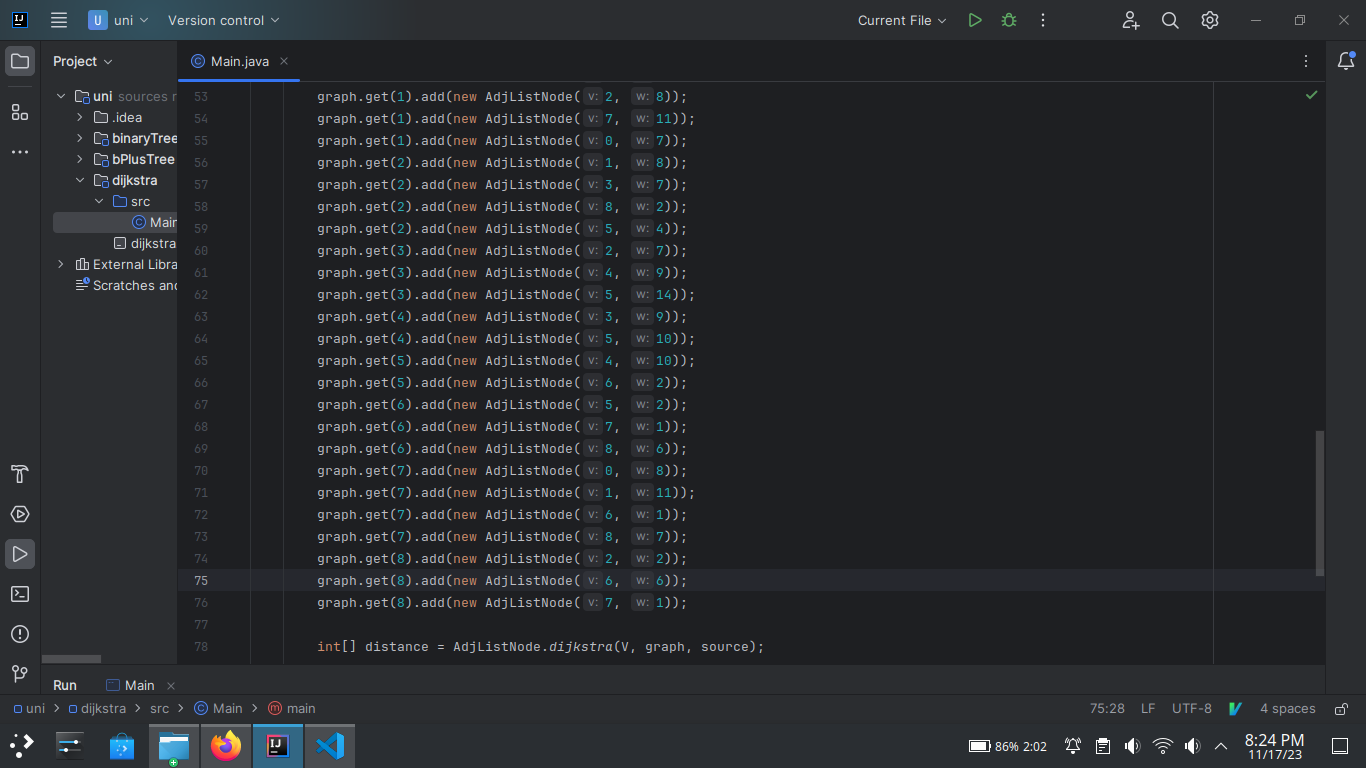
\includegraphics[scale=0.4]{../imgs/c3.png}
  \caption{code fragment 4}
  \label{fig:4}
\end{figure}

\begin{figure}[H]
  \centering
  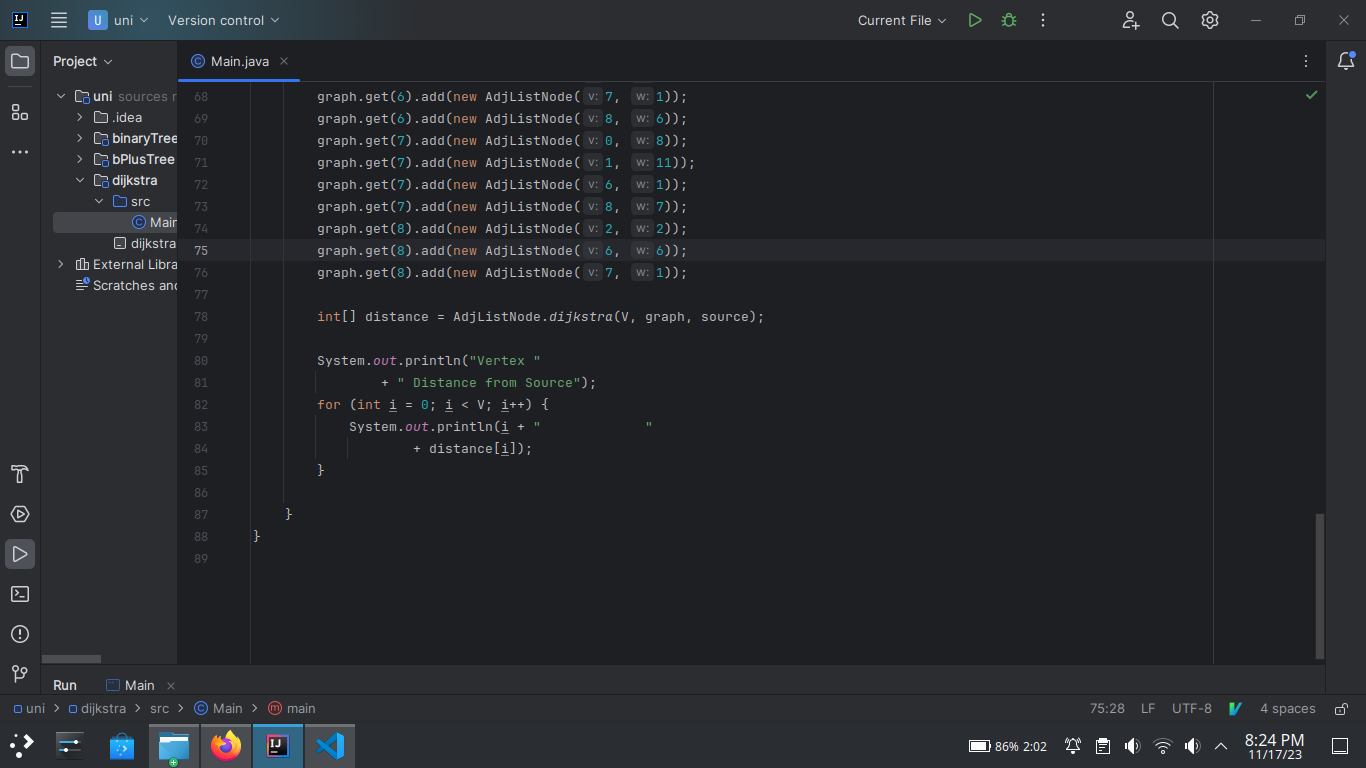
\includegraphics[scale=0.4]{../imgs/c4.png}
  \caption{code fragment 5}
  \label{fig:5}
\end{figure}



\section{Análisis de complejidad}
Por conteo de lineas obtenemos $O(2+V+3+ELogV+2V-1+V+1)$, donde las constantes pues son las constantes
el primer V (que seria como la n en otros algoritmos) es por el Arrays.fill
luego el ELogV es por el while que analizado tiene ese comportamiento y lo restante es lo del ultimo if statement. \\
La complejidad temporal del código parece $O(V^2)$
ya que hay dos bucles while anidados. Si miramos más de cerca,
podemos observar que las declaraciones en el bucle interno se ejecutan $O(V+E)$
veces (similar a BFS). El bucle interno tiene una operación de 
 decreaseKey() que requiere un tiempo $O(LogV)$.
 Entonces, la complejidad del tiempo general es $O(E+V)*O(LogV)$, que es $O((E+V)*LogV) = O(ELogV)$
\section{Análisis de caminos mínimos}
El camino de campeche con ciudad victoria que es su capital más cercana con la frontera de USA tenemos el siguiente resultado
\\
Tiempo
\begin{figure}[H]
  \centering
  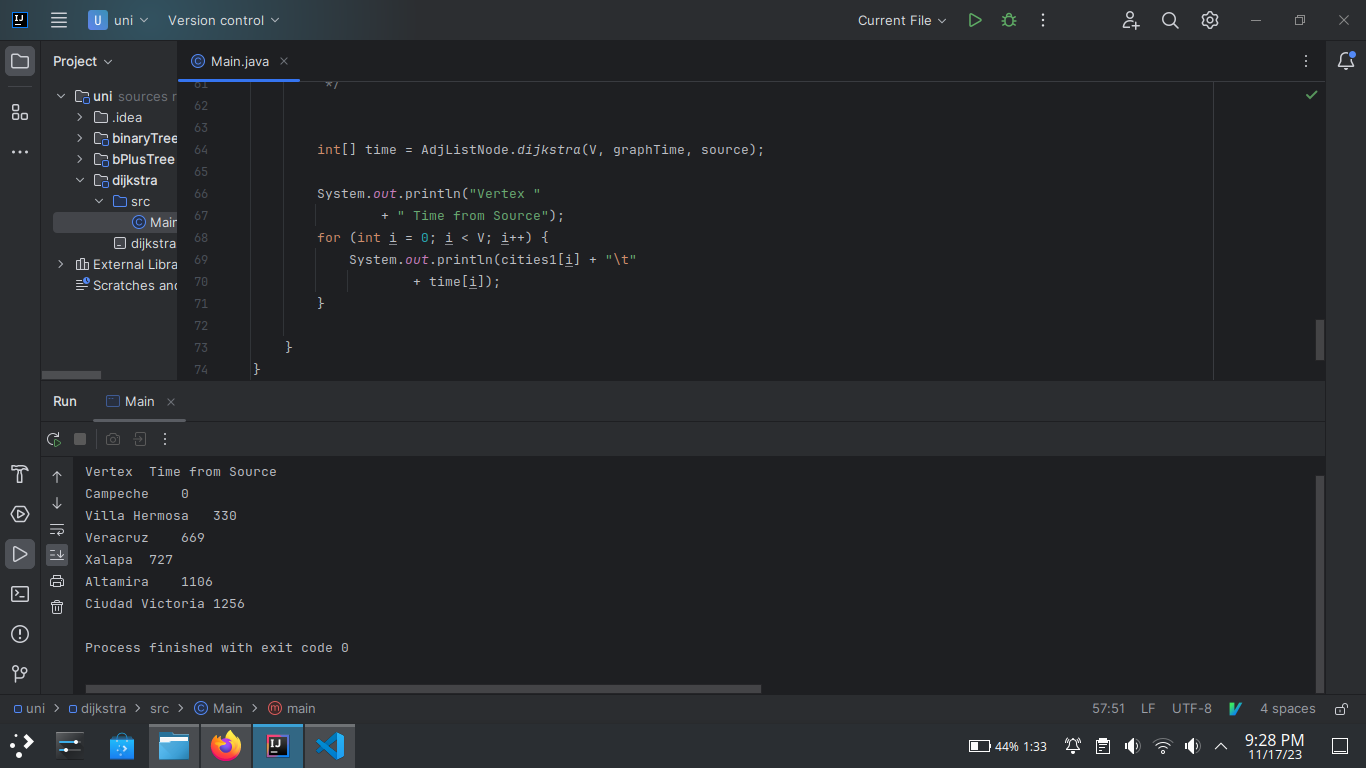
\includegraphics[scale=0.3]{../imgs/campeche.png}
  \caption{time}
  \label{fig:6}
\end{figure}

el tiempo esta en minutos por lo que si ponemos una calculadora de minutos a hora, nos da un total de 21 hrs prácticamente.
\\
Distancia
\begin{figure}[H]
  \centering
  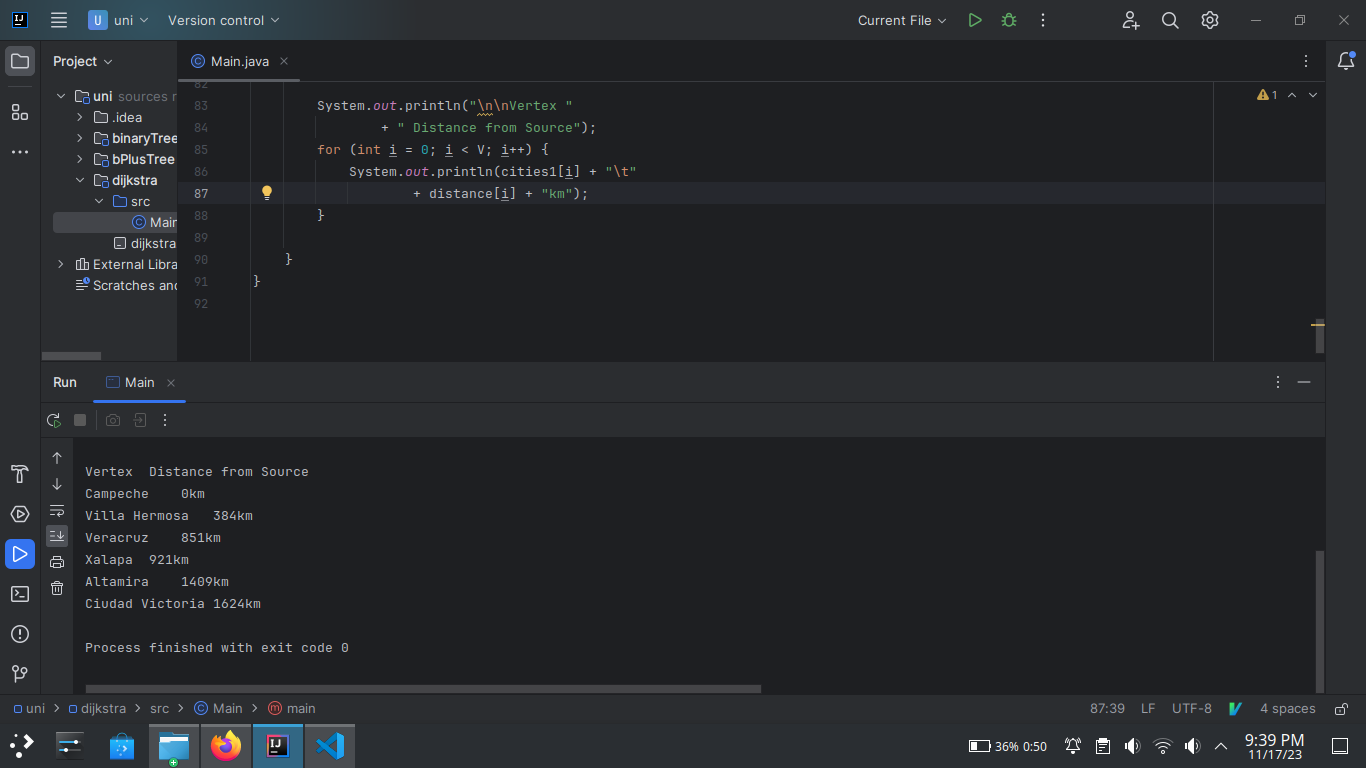
\includegraphics[scale=0.3]{../imgs/campeche1.png}
  \caption{time}
  \label{fig:7}
\end{figure}

En la figura \ref{fig:7} ya nos da el resultado final: 1624 km
\\
Ahora con tuxtla gutierrez chiapas que termina siendo casi lo mismo

\begin{figure}[H]
  \centering
  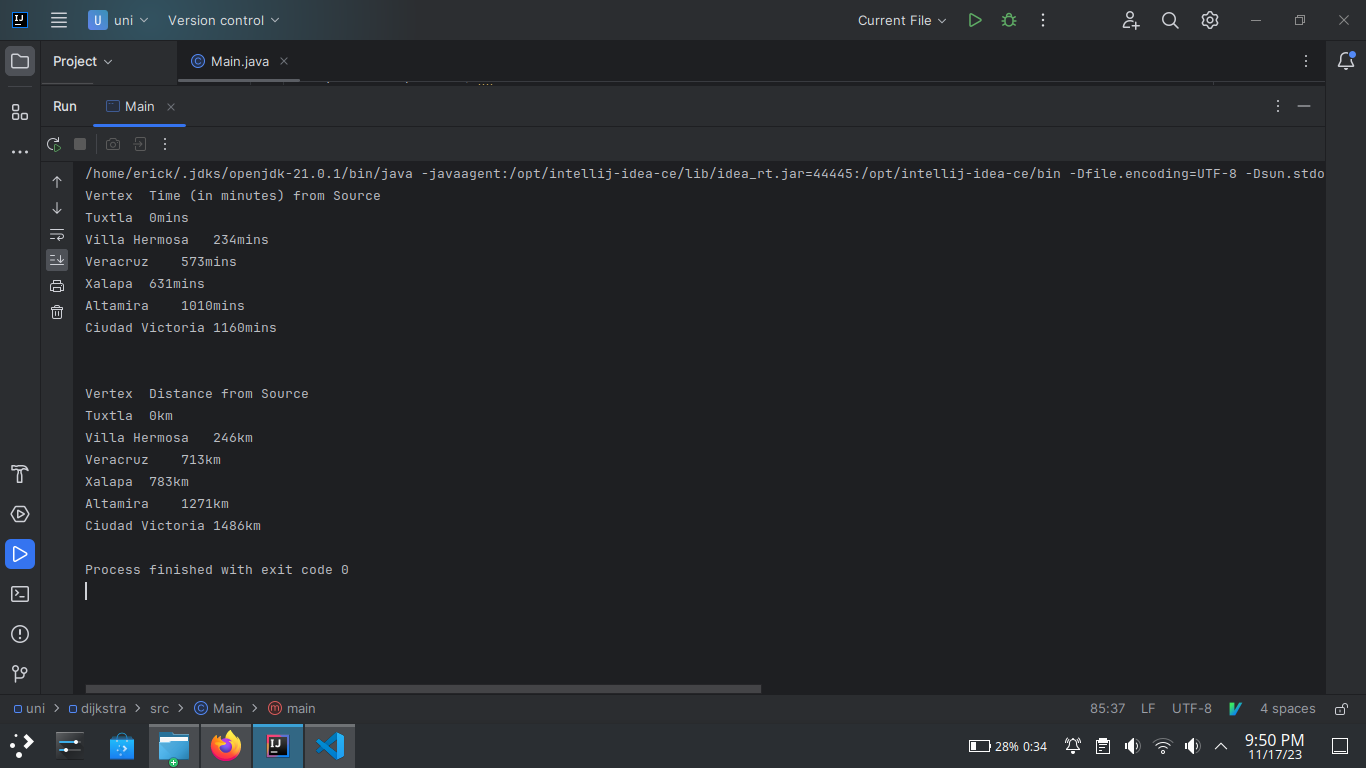
\includegraphics[scale=0.3]{../imgs/tux.png}
  \caption{time \& distance}
  \label{fig:8}
\end{figure}
Guerrero(chilpancingo)

\begin{figure}[H]
  \centering
  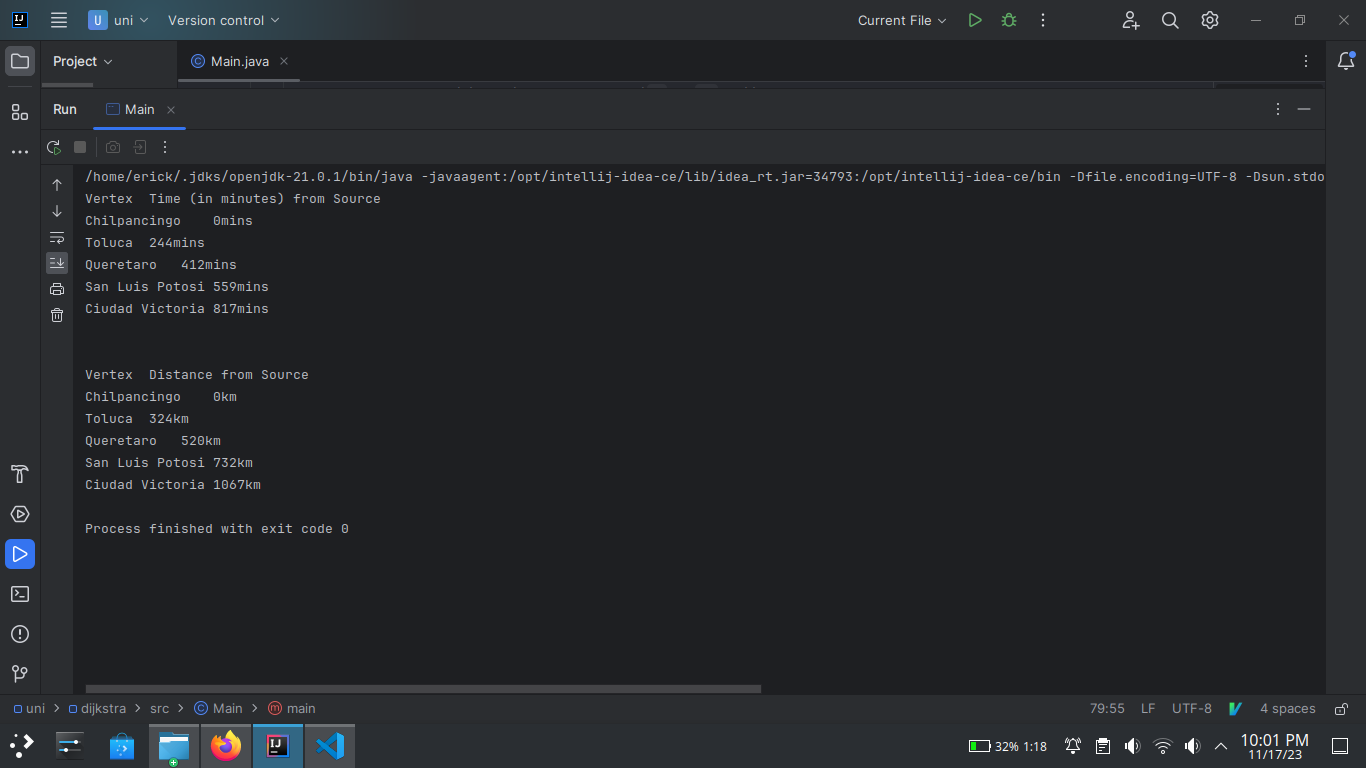
\includegraphics[scale=0.3]{../imgs/chil.png}
  \caption{time \& distance}
  \label{fig:9}
\end{figure}
Oaxaca(Oaxaca de Juarez)

\begin{figure}[H]
  \centering
  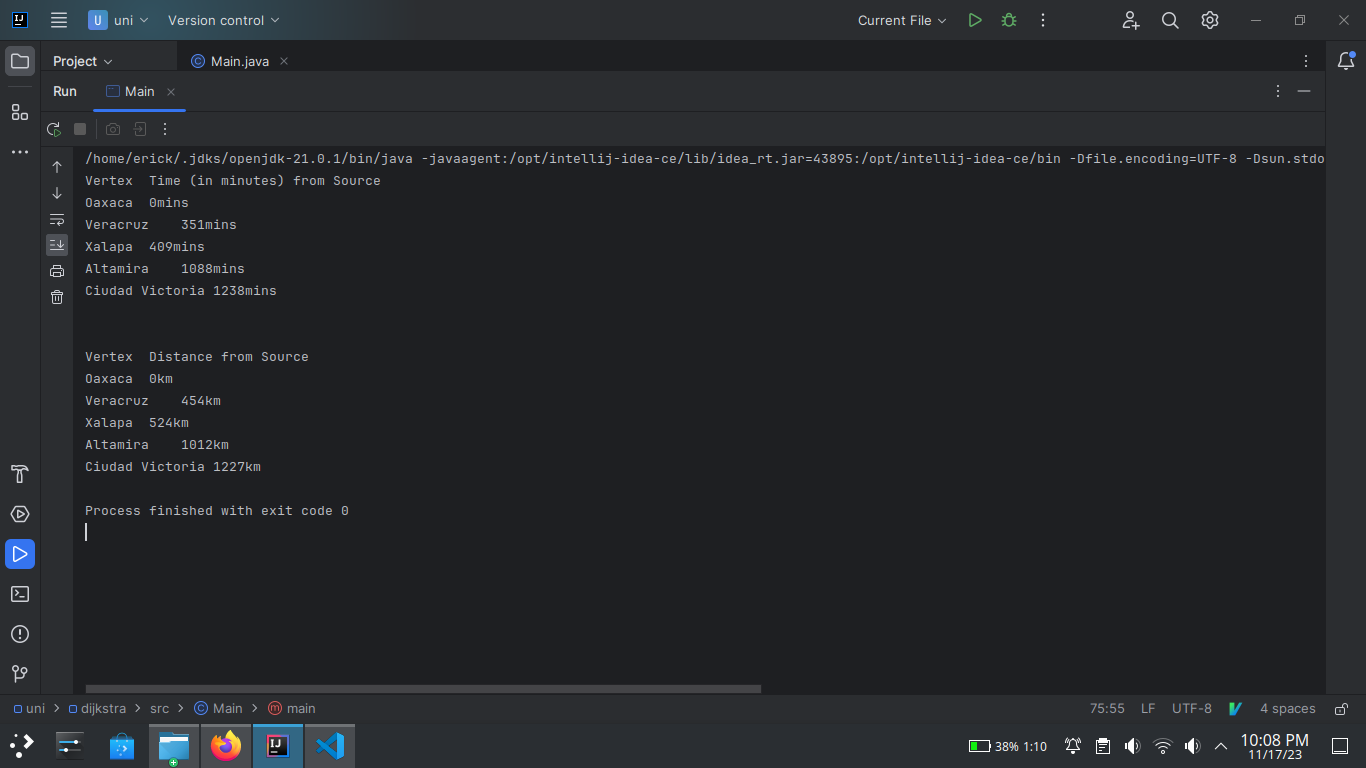
\includegraphics[scale=0.3]{../imgs/oaxaca.png}
  \caption{time \& distance}
  \label{fig:10}
\end{figure}
Quintana Roo(Chetumal)

\begin{figure}[H]
  \centering
  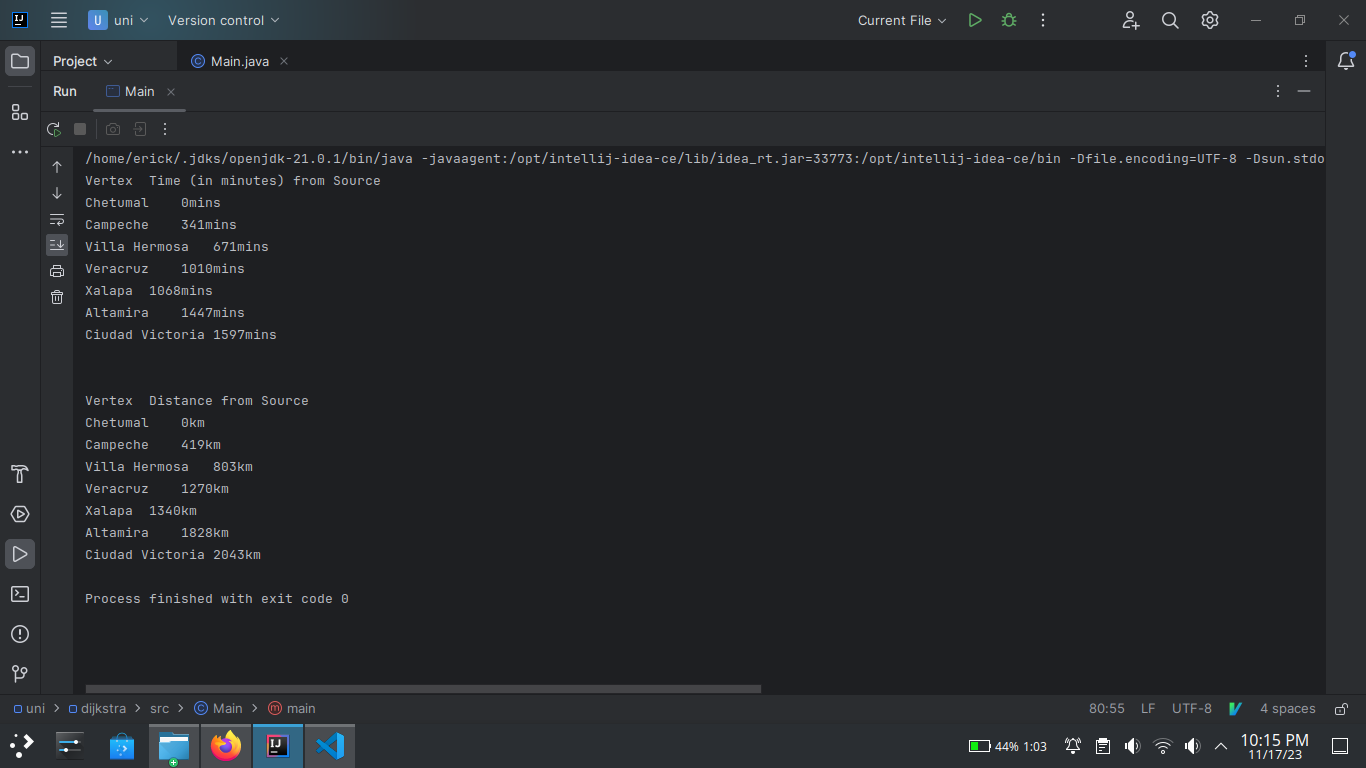
\includegraphics[scale=0.3]{../imgs/chetu.png}
  \caption{time \& distance}
  \label{fig:11}
\end{figure}
Tabasco(Villa hermosa)

\begin{figure}[H]
  \centering
  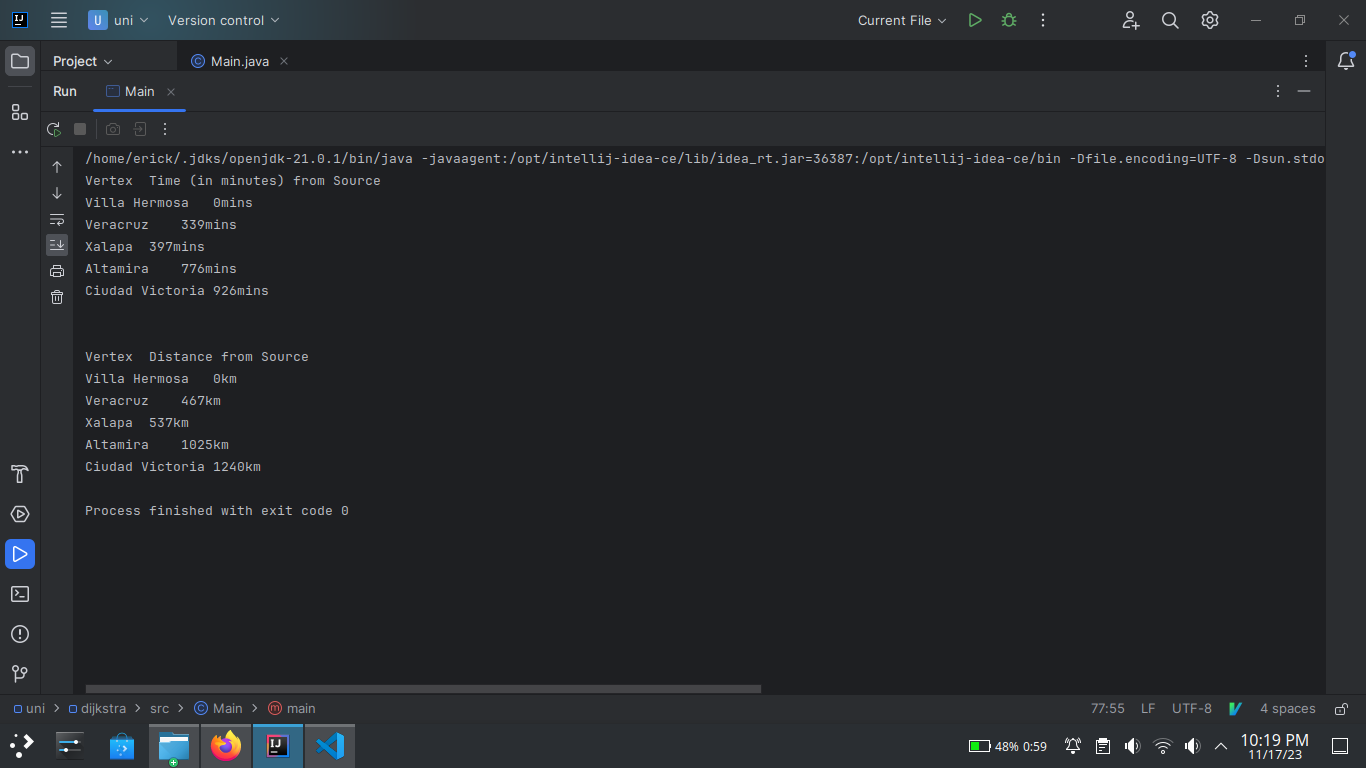
\includegraphics[scale=0.3]{../imgs/vh.png}
  \caption{time \& distance}
  \label{fig:12}
\end{figure}
Yucatan(merida)

\begin{figure}[H]
  \centering
  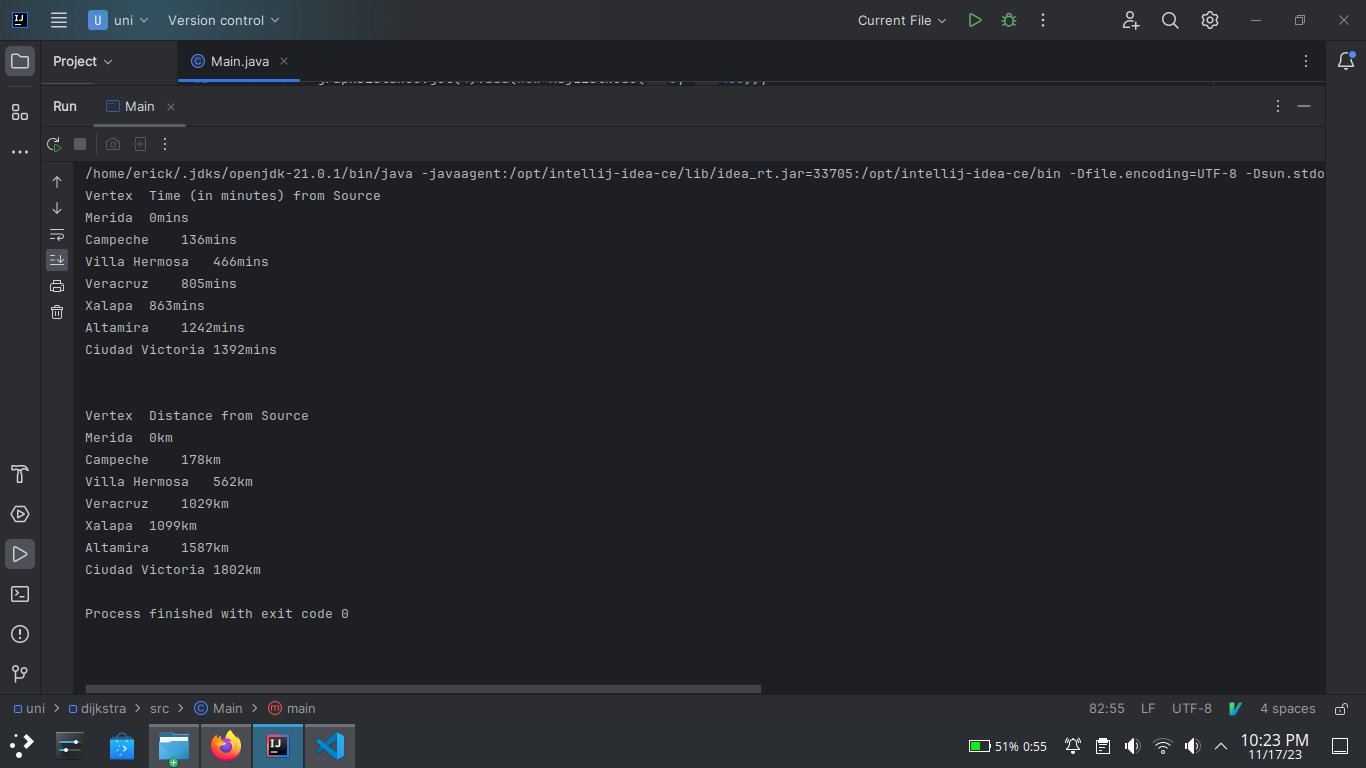
\includegraphics[scale=0.3]{../imgs/merida.png}
  \caption{time \& distance}
  \label{fig:13}
\end{figure}

Ahora analizaremos los estados con mayor IDH

CDMX

\begin{figure}[H]
  \centering
  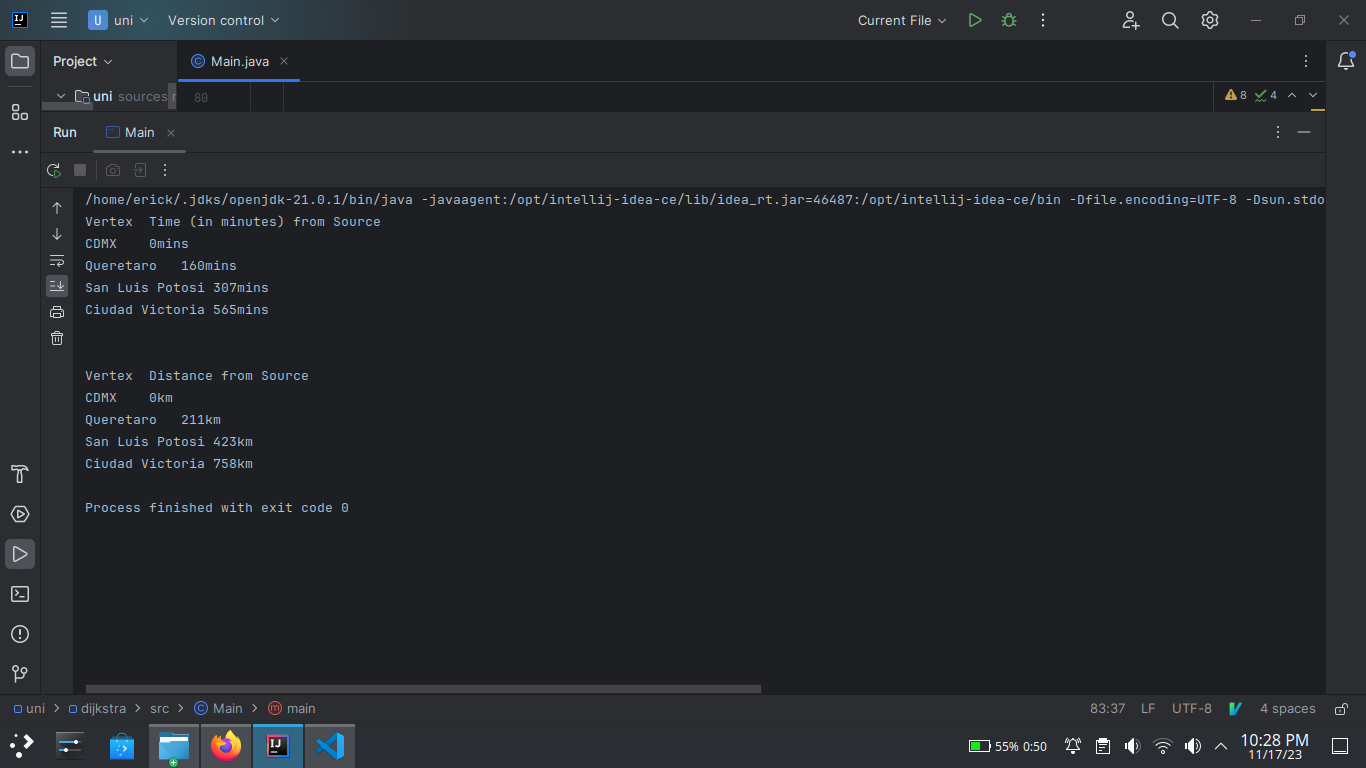
\includegraphics[scale=0.3]{../imgs/cdmx.png}
  \caption{time \& distance}
  \label{fig:14}
\end{figure}

Nuevo Leon(Monterrey), este ya es una frontera
\\
Baja California(Mexicali), igual, ya es una frontera
\\
Aguascalientes

\begin{figure}[H]
  \centering
  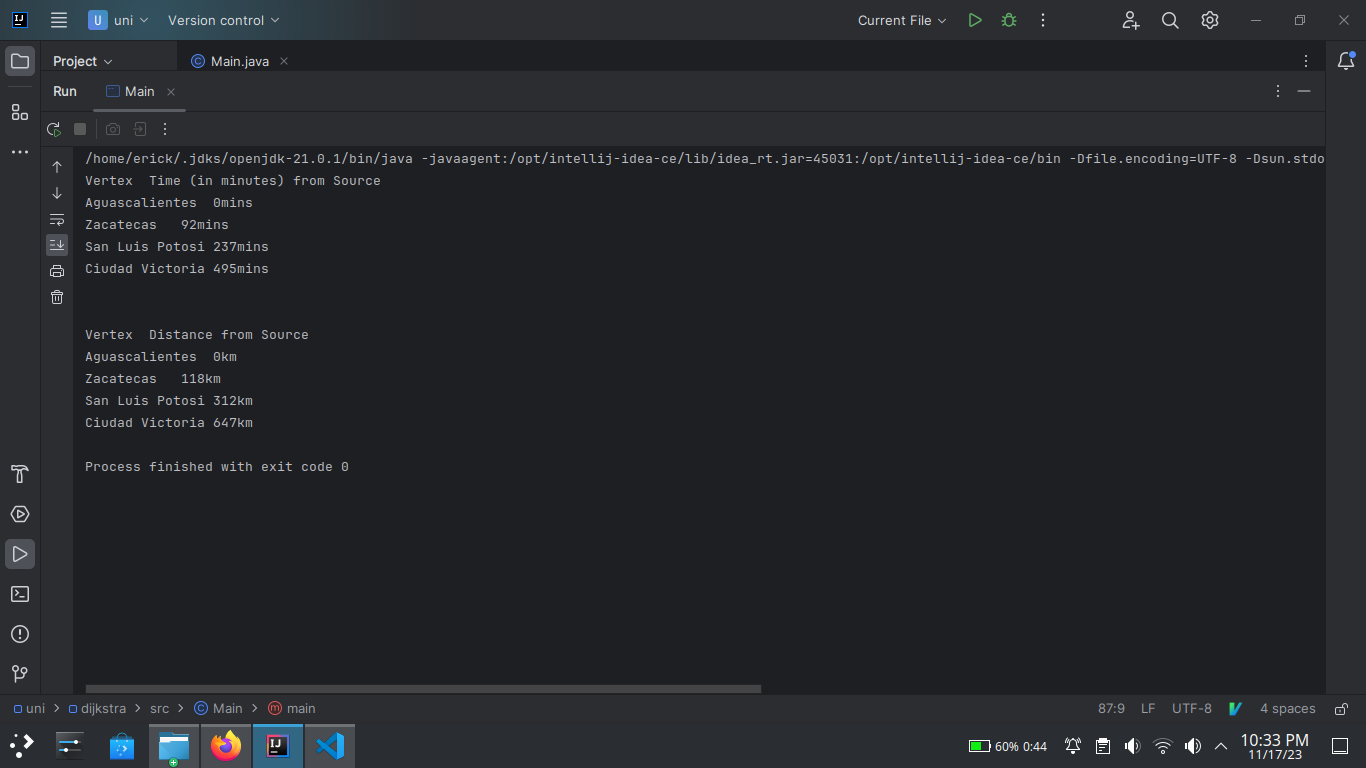
\includegraphics[scale=0.3]{../imgs/aguas.png}
  \caption{time \& distance}
  \label{fig:15}
\end{figure}

Baja California Sur (La Paz)


\begin{figure}[H]
  \centering
  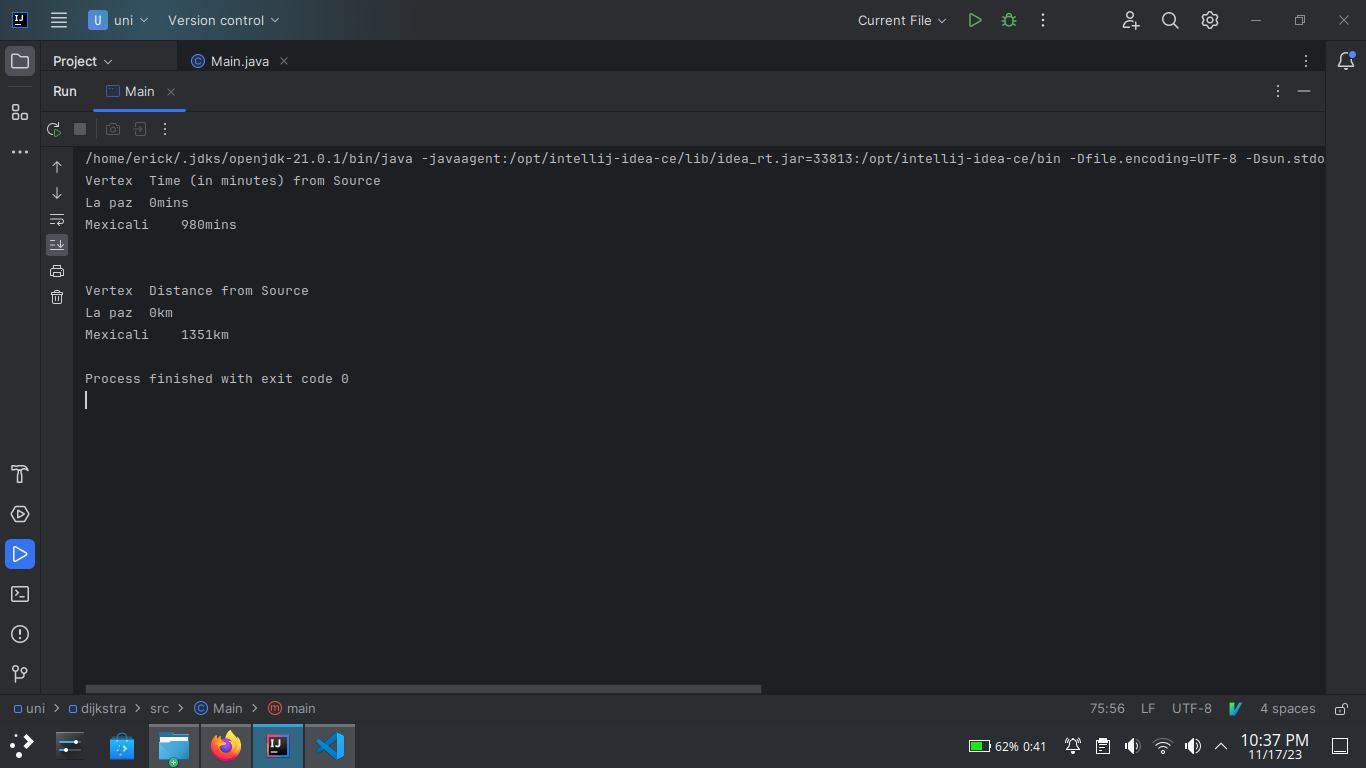
\includegraphics[scale=0.3]{../imgs/bcsur.png}
  \caption{time \& distance}
  \label{fig:16}
\end{figure}

\subsection*{análisis}
Tomando en cuenta que el promedio de velocidad que también lo calculan los softwares
de google maps son muy precisos y como se tomo el tiempo de ahi podemos simplemente concluir que 
a nuestro sureste del país le queda muy inaccesible la frontera con USA y es simple comparación. 

\section{Conclusiones}\label{Conclusiones}				% -------------------- Conclusiones
Nota: abajo de las conclusiones se encuentran los puntos extras
\\
Yo considero que esto afecta levemente debido a que no estamos considerando el comercio del mar 
en esta problemática sin embargo plantear una solución a la falta de conexiones no es nada fácil,
simplemente añadir que hacer carreteras lo mas estrechas posibles ayuda mucho y podría reducir tiempo 
y gasolina para cualquier vehículo.



\section{puntos extras}

\begin{figure}[H]
  \centering
  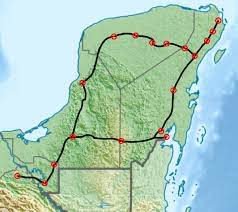
\includegraphics[scale=0.9]{../imgs/Untitled.jpg}
  \caption{tren maya}
  \label{fig:17}
\end{figure}

En mi opinion el comercio mejora insignificantemente debido a dos razones muy simples
\begin{itemize}
  \item El tren se esta construyendo para turistas:
  Estoy seguro de que el tren si va a tener "vagones" para transportar muchos productos, etc 
  no obstante su primordial rol es mover al turismo entre estos estados cuyo poder viene del turismo
  esto si influye muy positivamente al mercado sobre todo a la economía, pero cuando se trata de 
  transporte no vemos mucha diferencia, el tren va a poder ser mas rápido que un coche, pero este 
  es muy limitado y no sabemos aun el producto final de este gran proyecto. 
  \item Las rutas no cambian mucho
  pese a que con una via de tren yo la puedo poner logrando muchas intersecciones, estas siguen 
  estando situadas en el sureste del país sin llegar tan lejos donde solo en ese caso ya podríamos
  notar un poco mas de mejora ya que los estados con mas conexiones se encuentran todavía mas al centro
  del país.
\end{itemize}




  \end{document}	
